\documentclass[border=0.8ex,svgnames,varwidth]{standalone}
\usepackage{amsmath,mathtools}
\usepackage{fontspec}
\setmainfont{Source Serif 4}
\setsansfont{Source Sans 3}
\setmonofont{Source Code Pro}
\usepackage{subcaption}
\usepackage{tikz}
\usetikzlibrary{positioning,calc}
\captionsetup{
  font=scriptsize,
  labelfont=it,
  textfont=rm,
  labelformat=parens,
  position=above,
  labelsep=space,
  justification=centering,
}
\begin{document}
\begin{figure}
  \centering
  \begin{subfigure}[b]{.48\linewidth}
    \centering
    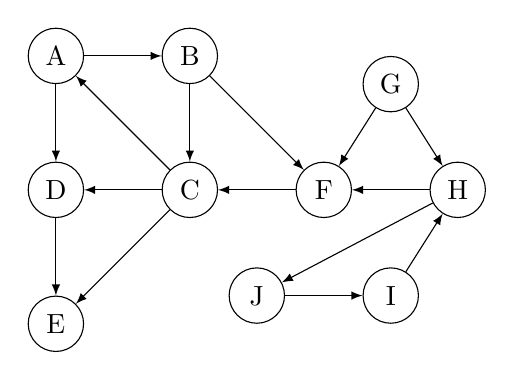
\begin{tikzpicture}[
      node distance=2.8em,
      every node/.style={draw,circle,minimum size=2em},
      every path/.style={draw,>=latex},
      ]
      \coordinate(digraph);
      \node[below=1ex of digraph] (digraphA) {A};
      \node[right=of digraphA]   (digraphB) {B};
      \node[below=of digraphB]   (digraphC) {C};
      \node[below=of digraphA]   (digraphD) {D};
      \node[below=of digraphD]   (digraphE) {E};
      \node[right=of digraphC]   (digraphF) {F};
      \node[right=of digraphF]   (digraphH) {H};
      \node[above=of $(digraphF)!0.5!(digraphH)$] (digraphG) {G};
      \node[below=of $(digraphC)!0.5!(digraphF)$] (digraphJ) {J};
      \node[below=of $(digraphF)!0.5!(digraphH)$] (digraphI) {I};
      \path[->]
      (digraphA) edge (digraphB)
      (digraphA) edge (digraphD)
      (digraphB) edge (digraphC)
      (digraphB) edge (digraphF)
      (digraphC) edge (digraphA)
      (digraphC) edge (digraphD)
      (digraphC) edge (digraphE)
      (digraphD) edge (digraphE)
      (digraphF) edge (digraphC)
      (digraphG) edge (digraphF)
      (digraphG) edge (digraphH)
      (digraphH) edge (digraphF)
      (digraphH) edge (digraphJ)
      (digraphJ) edge (digraphI)
      (digraphI) edge (digraphH);
    \end{tikzpicture}
    \caption{digraph}
  \end{subfigure}
  \hfill
  \begin{subfigure}[b]{.48\linewidth}
    \centering
    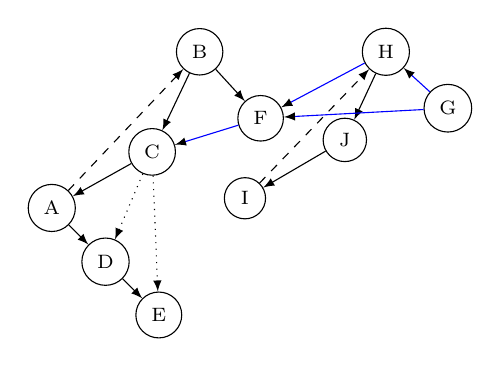
\begin{tikzpicture}[
      node distance=1.8em,
      every node/.style={draw,circle,minimum size=1em,font=\scriptsize},
      every path/.style={draw,>=latex},
      ]
      \coordinate(dfst);
      \node(dfstB) {B};
      \node[below right=1.2em and 1em of dfstB] (dfstF) {F};
      \node[below left=2.4em and .5em of dfstB] (dfstC) {C};
      \node[below left=.8em and 2.4em of dfstC] (dfstA) {A};
      \node[below right=1em of dfstA] (dfstD) {D};
      \node[below right=1em of dfstD] (dfstE) {E};
      \node[right=5em of dfstB] (dfstH) {H};
      \node[below left=2em and .3em of dfstH] (dfstJ) {J};
      \node[below left=1em and 2.5em of dfstJ] (dfstI) {I};
      \node[below right=.8em and 1em of dfstH] (dfstG) {G};
      \path[->]
      (dfstB) edge (dfstC)
      (dfstB) edge (dfstF)
      (dfstC) edge (dfstA)
      (dfstA) edge (dfstD)
      (dfstD) edge (dfstE)
      (dfstH) edge (dfstJ)
      (dfstJ) edge (dfstI);
      \path [dashed,->]
      (dfstA) edge (dfstB)
      (dfstI) edge (dfstH);
      \path [dotted,->]
      (dfstC) edge (dfstD)
      (dfstC) edge (dfstE);
      \path [draw=Blue,->]
      (dfstF) edge (dfstC)
      (dfstH) edge (dfstF)
      (dfstG) edge (dfstF)
      (dfstG) edge (dfstH);
    \end{tikzpicture}
    \caption{DFS tree}
  \end{subfigure}
\end{figure}
\end{document}
